% -----------------------------------------
\chapter{Materiais e Métodos}\label{chp:LABEL_CHP_3}
% -----------------------------------------
Neste capítulo serão apresentados os materiais e métodos utilizados para o desenvolvimento da aplicação. As linguagens de programação, os frameworks, bibliotecas e suas especificações técnicas são apresentados em \ref{materiais}. Como serão utilizados tais materiais e os passos para o desenvolvimento da aplicação são descritos em \ref{metodos}.

\section{Materiais} \label{materiais}
A seguir, serão descritos os materiais utilizados para o desenvolvimento da aplicação, que envolvem os frameworks web front e backend do projeto e suas linguagens de programação, juntamente com a descrição das tecnologias do SGBD e versionamento.

\subsection{HTML}
O Hiper Text Markup Language (HTML) é uma linguagem de marcação utilizada para o desenvolvimento de páginas web na qual permite a inserção de conteúdo, estabelece a estrutura básica, assim como a organização de informações de uma página web. Isto o torna o componente básico da web, juntamente ao CSS e JavaScript, sendo um conjunto de elementos conectados formando informações das mais variadas, podendo conter palavras, imagens, documentos entre outros tipos dados. Seu funcionamento se dá pela leitura de seus arquivos, que é renderizada para o usuário final por meio de um navegador web. Portanto, é o esqueleto no qual uma página se forma \cite{FLANAGAN}.

\subsection{CSS}
O Cascading Style Sheets (CSS) é a linguagem utilizada para estilizar o HTML. Todos os elementos podem ser estilizados, ou seja, é possível modificar detalhes como espaçamentos, cores, margens, fonte, tamanho desta fonte, bordas, efeitos visuais, entre vários outros detalhes para cada um. Desta maneira, é um complemento ao HTML, dando forma e modificação desta estrutura previamente feita \cite{FLANAGAN}.

Segundo \citeonline{DUCKETT}, o CSS pode ser reutilizado em diversas páginas criando padrões visuais a aplicação, assim como utilizado em áreas específicas. Torna as páginas, desde que usado para este princípio, mais responsivas ao organizar o layout e adaptar cada bloco visual para telas com diferentes tamanhos.

\subsection{JavaScript}
Segundo \citeonline{ROBBINS} JavaScript é a linguagem de programação da web, que é interpretada pelos navegadores web. Diversos sites modernos utilizam esta linguagem para manipular o comportamento da página em conjunto ao HTML e CSS. Podendo ser utilizada tanto no frontend quanto no backend se torna muito versátil para o desenvolvimento destes sistemas. A mudança de dados sem a necessidade de recarregar toda a página permite uma flexibilidade na qual dados podem carregar independentes e de forma assíncrona sem que tenha a necessidade de um usuário final estar constantemente monitorando qualquer alteração \cite{FLANAGAN}.

Existem diversas bibliotecas para a linguagem com funções pré-prontas que visam a agilidade no desenvolvimento, que lidam, por exemplo, com a reatividade na página, como é o caso do React.js. Os frameworks tem o há incluso nas bibliotecas juntamente as suas regras de implementação, como é visto no Next.js e sua estruturação das páginas contendo o React.js entre as suas bibliotecas \cite{ROBBINS}.

\subsection{Typescript}
O TypeScript é uma linguagem de programação de código aberto desenvolvido pela Microsoft e é um conjunto de ferramentas e boas práticas de programação para JavaScript, o qual adiciona recursos a esta linguagem. Dentre as adições, vale ressaltar a tipagem estática, visto que JavaScript não suporta isto \cite{TYPESCRIPT}.A orientação a objetos também é suportada pelo TypeScript, o que possibilita a criação de interfaces para os objetos. Sua utilização pode ser atrelada ao JavaScript, ou seja, podem ser utilizados em conjunto para uma maior flexibilidade \cite{CHERNY}.

\subsection{PHP}
O PHP é uma linguagem de script open-source de uso geral, muito utilizada, e especialmente adequada para o desenvolvimento web e que pode ser embutida dentro do HTML. Muito utilizada para o backend, esta linguagem tem evoluído rapidamente, sendo suportada por diversos desenvolvedores ao redor do mundo. Além disso, o PHP moderno engloba muitas práticas novas que podem ser desconhecidas para aqueles que são novos na linguagem ou para aqueles que estão atualizando de suas versões anteriores \cite{LOCKHART}.

\subsection{Laravel}
Framework é um conjunto de ferramentas, recursos e funcionalidades que visa facilitar e agilizar tarefas mais comuns no desenvolvimento de sistemas, e é criado em uma determinada linguagem de programação. O framework escolhido foi o Laravel, feito com base no PHP, é gratuito e possui código aberto. Este é utilizado no desenvolvimento de sistemas web e seu objetivo é fornecer código e recursos claros, simples e bonitos que ajudem os desenvolvedores a aprender, iniciar e desenvolver rapidamente e escrever um código simples, claro e duradouro \cite{STAUFFER}. A hospedagem do Laravel é suportada por diversos provedores, incluindo o Heroku, que será detalhado nesta seção. 

O Laravel foi baseado no padrão de projeto Model, View, Controller (MVC), que divide a aplicação em três camadas, sendo estas:
\begin{itemize}
    \item \textbf{Modelo:} dita as regras de negócio e os dados da aplicação.
    \item \textbf{Visão:} exibição dos dados para o usuário.
    \item \textbf{Controlador:} interpreta as entradas do usuário para as outras camadas de acordo com o que foi solicitado.
\end{itemize}

A escolha para o projeto se deve ao fato de que, de acordo com a figura \ref{framework_popular}, o Laravel é o framework backend mais popular até março de 2021 segundo dados dos repositórios com mais estrelas do GitHub, e isto se deve a diversas características que estão contidas nele, sendo estas:

\begin{figure}[H]
    \caption{\label{framework_popular}Frameworks backend mais populares}
    \vspace{5pt}
    \centering
    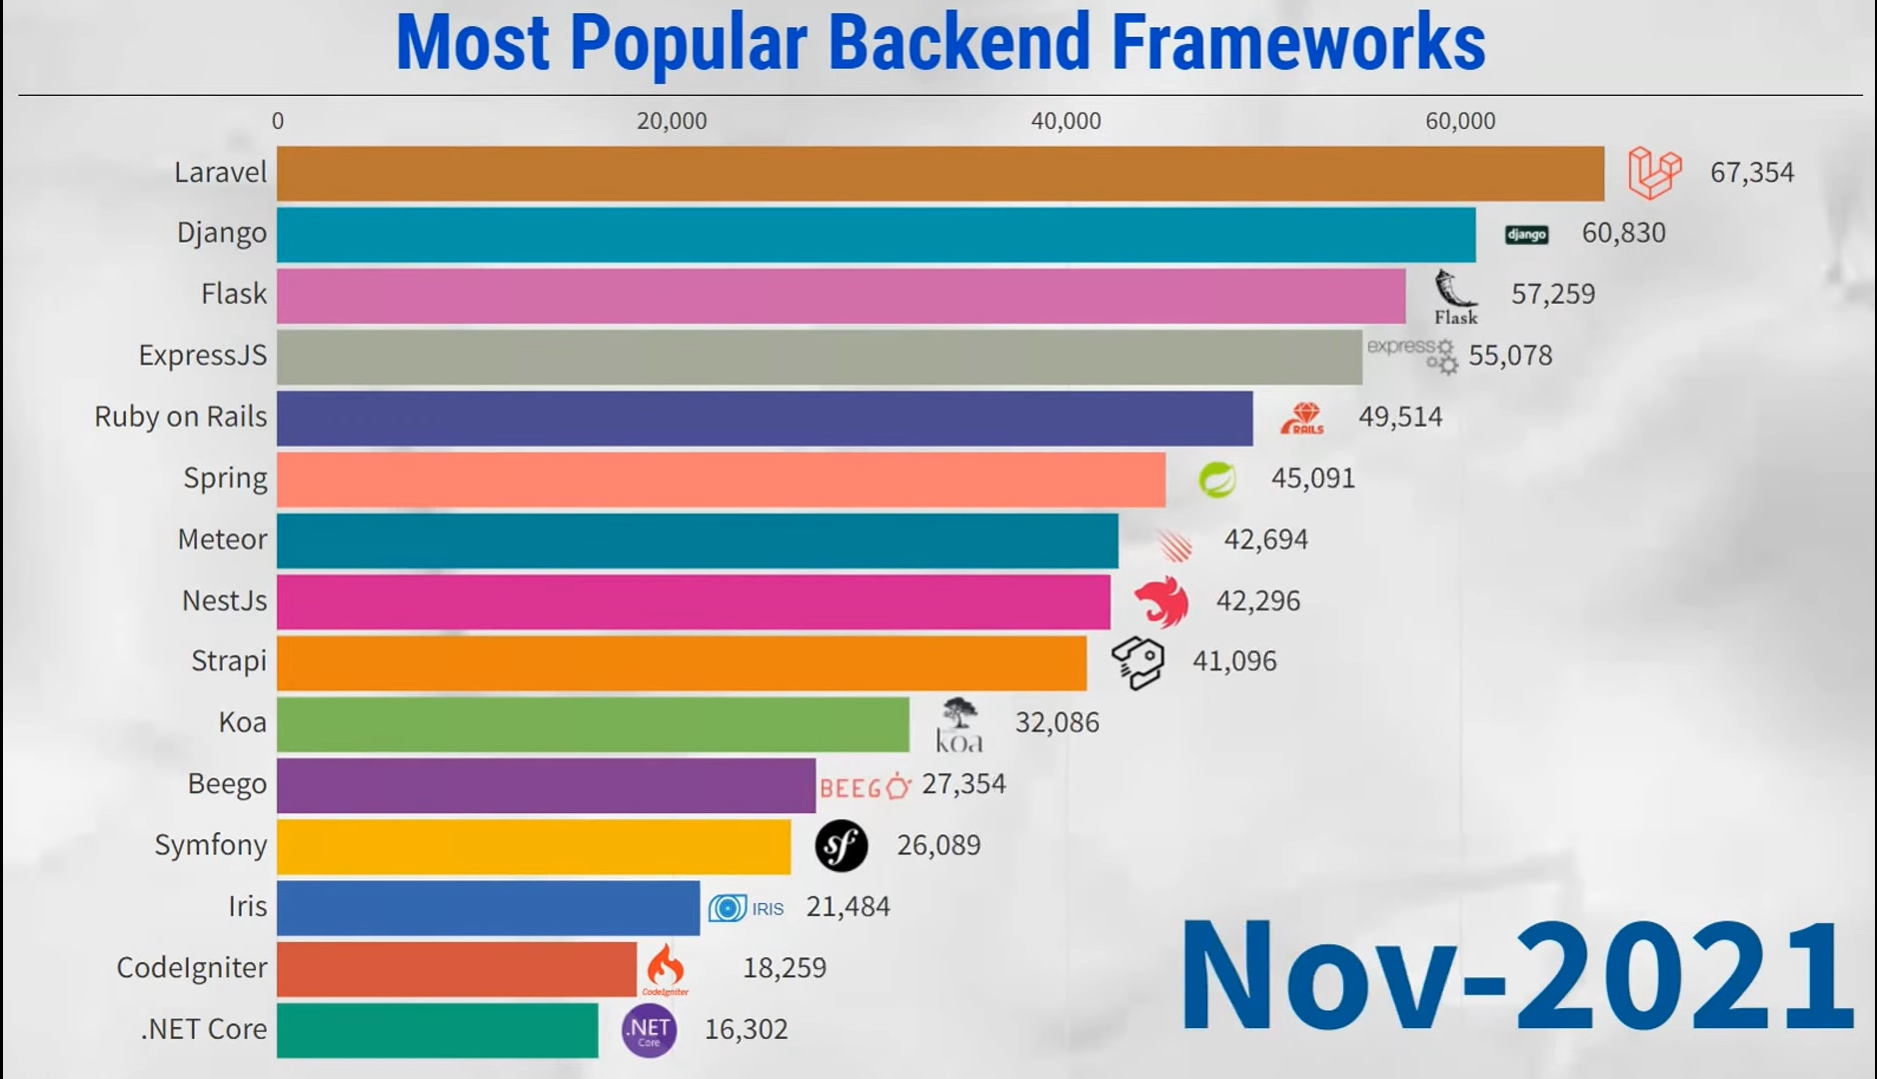
\includegraphics[scale=.20]{laravel.png}
    \vspace{5pt}
    \legend{Fonte: Statistcs and data\cite{STATISTICS}}
\end{figure}

\begin{itemize}
    \item \textbf{Roteamento rápido e simples:} é possível criar rotas com segurança e de forma simples, evitando requisições não autorizadas de maneira simples por meio dos verbos GET, POST, PUT e DELETE. Também é possível criar grupos de rotas com permissões de acesso específicas.
    \item \textbf{ORM Eloquent:} este facilita a interação com o banco de dados utilizando cada tabela como um objeto modelo correspondente. Outra facilidade é a forma de interação com as tabelas, que seriam a recuperação de registros do banco de dados, assim como sua inserção, atualização e exclusão.
    \item \textbf{Migration:} As migrations são como o controle de versão do banco de dados, sendo estas as definições de criação e alteração do schema, podendo ser revertidas caso necessário.
    \item \textbf{Transmissão de eventos em tempo real:} utilizando da tecnologia de WebSockets, é possível atualizar em tempo real e constantemente a interface do usuário enviando dados sempre que determinado evento ocorra.
\end{itemize}

\subsection{SQL}
A linguagem SQL é utilizada para executar tarefas em tabelas de banco de dados. Ou seja, com os comandos de inserção, deleção, atualização e leitura de dados é possível manipular as informações por meio de comandos de consulta com diversas informações contidas \cite{HEUSER}. Suas principais características são:
\begin{itemize}
    \item \textbf{Query:} é possível solicitar informações específicas de um banco de dados.
    \item \textbf{Manipulação de dados:} adicionar, excluir, alterar, ordenar, requisitar além outras operações para os registros contidos no banco de dados.
    \item \textbf{Acesso de controle de dados:} fornece técnicas de segurança para proteger dados, limitando quais usuários podem controlar e limitar o que podem fazer com os registros contidos dentro do banco de dados.
\end{itemize}
\subsection{Git}
Controlador de versão é uma ferramenta de software na qual ajuda os desenvolvedores, seja em equipe ou não, a gerenciar alterações no código-fonte, mantendo o registro destas modificações. Então, o GIT é um sistema de controle de versão que possui código aberto, é flexível (possui vários tipos de fluxos de trabalho de desenvolvimento não lineares), é seguro (toda sua estrutura é protegida com um algoritmo de hash de criptografia seguro chamado SHA1) e possui um bom desempenho (Fazer o commit de novas alterações, branches, mesclagem e comparação de versões anteriores – tudo é otimizado para desempenho) \cite{SANTACROCE}.

\subsection{Bootstrap}
Para a estilização do frontend foi escolhido o Bootstrap, que é um framework gratuito de HTML, CSS e JavaScript no qual visa a criação de sites responsivos, ou seja, se adaptando tanto para telas maiores, como monitores de computador assim como para telas menores, como é o caso dos celulares. Além disso, contém bibliotecas prontas de estilização que procuram agilizar o processo de desenvolvimento no CSS e JavaScript, assim como a reutilização do código e sua personalização \cite{SPURLOCK}.

Este possui um sistema de grid, que resultou em sua responsividade, e dimensiona a aplicação em até doze colunas de acordo com o tamanho de cada dispositivo. Além disso possui componentes de interface que agilizam o desenvolvimento, visto que já estão implementados de forma que podem ser personalizados, sendo um exemplo a barra de navegação (navbar).

\subsection{React}
Para melhorar a interatividade da interface do usuário, foi escolhido o React, que segundo seus próprios criados é “uma biblioteca JavaScript declarativa, eficiente e flexível para a criação de interfaces de usuário (UI)”. Isso quer dizer que é uma coleção de funcionalidades que podem ser utilizadas e reutilizadas pelo desenvolvedor, que são seus componentes. Isto permite uma padronização na interface, além de reaproveitamento de código \cite{ZAMMETTI}.

A criação de views é facilitada e simples, sendo estas atualizadas e renderizadas apenas para os componentes necessários à medida que os dados forem alterados, sendo estas declarativas fazendo que o código seja mais simples de se depurar.

Sua forma de trabalhar é com componentes encapsulados gerenciadores dos seus próprios estados, que combinados formam uma UI complexa, podendo ser escritos em JavaScript ou TypeScript.

\subsection{Next.js}
O Next.js é um framework do React, o qual adiciona várias funcionalidades para esta biblioteca, visando acelerar o processo de desenvolvimento. Construído com intuito de melhorar o desempenho da aplicação implementada em React, há uma indexação do conteúdo da página e pelos motores de busca. Ou seja, se torna mais rápido e prático ao desenvolvedor, melhorando a experiência para o usuário final \cite{KONSHIN}.

As principais adições do Next.js em relação ao React segundo a \citeonline{VERCEL} são:
\begin{itemize}
    \item \textbf{Componente de imagem otimizado:} com este componente é possível redimensionar, otimizar e exibir imagens no formato WebP (desde que o navegador suporte) evitando o envio de imagens grandes para dispositivos menores, como os celulares. E tal otimização é feita sob demanda, ou seja, é feita conforme os usuários solicitam, além de serem carregadas na página de forma assíncrona, não penalizando o carregamento do restante.
    \item \textbf{Roteamento por páginas:} dentro do diretório pages no projeto é possível, por meio de criação de demais pastas neste, rotas aninhadas, rotas dinâmicas e uma fácil integração entre estas. No primeiro caso, a o diretório “pages/blog/index.js” é facilmente acessível digitando apenas /blog no final do endereço, e no segundo caso o caminho “pages/blog/[id].js” é acessível por qualquer valor no endereço após o caminho padrão, que é o blog, como por exemplo: exemplo.com/blog/1.
    \item \textbf{Pré-rendericação:} por padrão, o framework gera, para cada página, um HTML com um arquivo JSON de dados ao invés de ser tudo realizado pelo JavaScript via client-side. E isto faz com que um motor de busca tenha melhor performance, dada a geração pré-renderizada, ou seja, preparado para melhorar os resultados de um SEO\footnote{Search Engine Optimization é utilizado para criar uma estratégia que irá aumentar a posição de um site no ranking nos resultados dos motores de busca. Quanto maior a classificação, mais tráfego orgânico para uma página terá.}. Portanto, cada página HTML terá o mínimo de código JavaScript necessário, fazendo com que torne inteiramente dinâmica, por meio de sua execução somente quando necessário.
\end{itemize}

Dada a pré-renderização do Next.js, há duas formas as quais ele pode realizar tal recurso, podendo estas serem utilizadas em conjunto dada as necessidades de cada página do projeto. Uma das formas que pode ser utilizada é por meio da Static Generation, que recupera informação, caso seja necessário, de forma estática no momento de construção e gera uma página HTML que será colocada em cache no CDN. Isto faz com que o usuário final terá de esperar apenas o tempo de download e construção do HTML e não de todo conteúdo, previamente feito em JavaScript. Em rotas dinâmicas, podem ser construídas com cache de um determinado período, ou seja, a cada um minuto esta página pode ser novamente alterada sua construção caso haja alguma requisição nesta.

A Server-side Rendering, que diferentemente da geração estática, a página HTML é gerada a cada requisição. Como a página não pode gerar um cache no CDN, será mais lenta, porém estará sempre atualizada no momento da requisição. Entretanto, por mais que seja gerada em tempo de execução, o processamento é similar ao anterior, visto que a página é renderizada no próprio servidor, enviando-se apenas o HTML para o cliente final, com as funções em JavaScript necessárias, fazendo com que evite processamento no navegador do usuário, e fique apenas no servidor \cite{VERCEL}.

A Vercel, criadora do Next.js, suporta todos os recursos da linguagem em sua hospedagem (mais detalhes a frente).

\subsection{MySQL}
Para o banco de dados, foi escolhido o MySQL é um SGBD relacional de código aberto usado na maioria das aplicações gratuitas para gerir suas bases de dados que utiliza a linguagem SQL. Este possui um alto desempenho, sendo possível verificar uma grande quantidade de dados em pouco tempo, o que gera também a escalabilidade deste sistema \cite{HEUSER}.

\subsection{GitHub}
O GitHub é uma plataforma online onde são criados e hospedados repositórios GIT de projetos. Este sistema, visa facilitar o controle de versões de um software ou aplicação, funcionando em um formato de rede social para desenvolvedores \cite{SANTACROCE}. Além disso, é amplamente utilizada com mais de 56 milhões de desenvolvedores em 2020 conforme mostra a figura \ref{utilizacao_github}. Dito isso, esta plataforma será utilizada para manter as versões da aplicação no frontend e no backend.

\begin{figure}[H]
    \caption{\label{utilizacao_github}Utilização por linguagem do GitHub}
    \vspace{5pt}
    \centering
    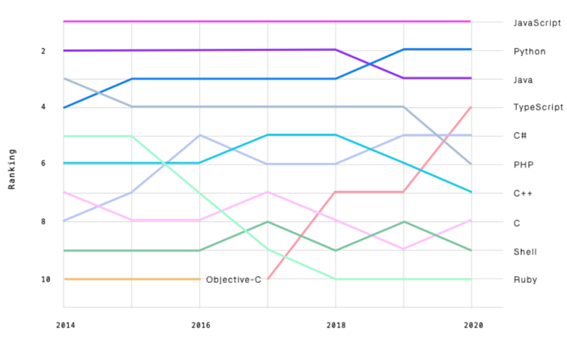
\includegraphics[scale=.75]{github.png}
    \vspace{5pt}
    \legend{Fonte: GitHub stats}
\end{figure}

\subsection{Gitflow}
Gitflow Workflow é um design de fluxo de trabalho Git que foi publicado e popularizado pela primeira vez por Vincent Driessen no nvie. Este define um modelo de ramificação rigoroso, projetado com base no lançamento do projeto, o que oferece uma estrutura robusta para gerenciar projetos maiores. O Gitflow é eficiente para projetos que possuem um ciclo de lançamento agendado, visto que não adiciona novos conceitos ao fluxo de trabalho, mas sim define funções específicas as ramificações e quando devem interagir (SANTACROCE, 2015). Ou seja, em conjunto com o versionamento do GitHub, será mais fácil localizar problemas, caso haja, assim como uma padronização em cada commit é também possível a verificação de o que foi feito de uma forma mais simples e rápida.

\subsection{Vercel}
A Vercel é uma plataforma que hospeda aplicações web frontend de forma gratuita por meio de um CDN\footnote{Central Delivery Network (Rede de Distribuição de Conteúdo) é uma rede de servidores que armazenam réplicas do conteúdo em memória cache do site e as entrega aos usuários visitantes, de acordo com sua localização geográfica de modo que os conecte no servidor mais rápido e mais próximo, fazendo com que se reduza a latência.}
global. Com seus 50 domínios disponíveis e 100Gb de largura de banda, juntamente com sua criptografia SSL fazendo a criptografia necessária dos dados para garantir a segurança. Além disso, há uma integração diretamente com o GitHub, que a cada commit na branch predeterminada é gerado um deploy, que atualizará o site com as últimas alterações. Sua escalabilidade é, segundo sua própria documentação, infinita, sendo que cada camada de sua infraestrutura aumenta e/ou diminui dinamicamente de acordo com o sistema e funções de armazenamento de cache necessários \cite{VERCEL}. 

Internamente na plataforma da Vercel, junto ao o seu framework Next.js, há uma otimização de imagem, que será carregada do servidor de acordo com a área de visualização do dispositivo, guardando-as em cache. Esta otimização reduz o uso de banda, minimizando o tráfego de rede de acordo com o que for necessário para o usuário, melhorando então a experiência geral de quem visita a aplicação.

\subsection{Firebase}
Para o armazenamento das imagens, será utilizado o Firebase Cloud Storage. Este oferece uma forma prática de salvar e recuperar arquivos, incluindo uma das utilizações das imagens, gerando uma url própria para uso. Contendo seu próprio sistema de regras de segurança e acesso como medida protetiva de seus arquivos, permite que apenas clientes autenticados se conectem. Com sua integração diretamente com o JavaScript, apenas a URL no banco de dados será salva, portanto sendo indexada diretamente nos servidores da Google.\cite{FIREBASE}

\subsection{Heroku}
O Heroku é uma plataforma como um serviço, que permite hospedagem, além de configurações e publicações de projetos na nuvem e, diferentemente da Vercel, integra também diversos bancos de dados e possui suporte ao PHP. Com sua integração com o GitHub, seu deploy do projeto é feito a cada commit registrado no sistema, o que facilita a integração. Além disto, esta plataforma é gratuita no seu início contendo uma máquina virtual com 512MB, podendo ser escalável à medida que for necessário com seus custos de infraestrutura. 

Segundo a plataforma,- é monitorado constantemente por múltiplos servidores a cada dependência, fazendo com que as correções sejam aplicadas assim que possível, tendo uma garantia ao usuário e seus servidores.  Outro detalhe é que a estabilidade em sua plataforma também é garantida por eles, visto que seus algoritmos internos verificam caso ocorra uma queda ou falha na aplicação em tempo de execução e a restaura como uma nova instância automaticamente, garantindo uma preservação dos serviços executados pelo seu usuário sem a necessidade de verificar constantemente o que está ativo \cite{HEROKU}.

\subsection{Tecnologias utilizadas}
Exemplificando a organização das tecnologias utilizadas, a figura \ref{info} demonstra a utilização e comunicação das tecnologias apresentadas nesta seção. No frontend está localizado na camada de visão da aplicação, que o usuário irá interagir, e então o framework Next.js, hospedado na Vercel e disponível em: \url{https://eventos-tcc.vercel.app/} irá fazer as requisições ao backend por meio de um webservice hospedado na Heroku. O backend irá processar a requisição da API, que por meio do Laravel, fará as consultas ao banco de dados, retornando uma resposta com os dados requisitados ao frontend para que sejam exibidos ao usuário por meio da interface gráfica.

\begin{figure}[H]
    \caption{\label{info}Organização das tecnologias utilizadas}
    \vspace{5pt}
    \centering
    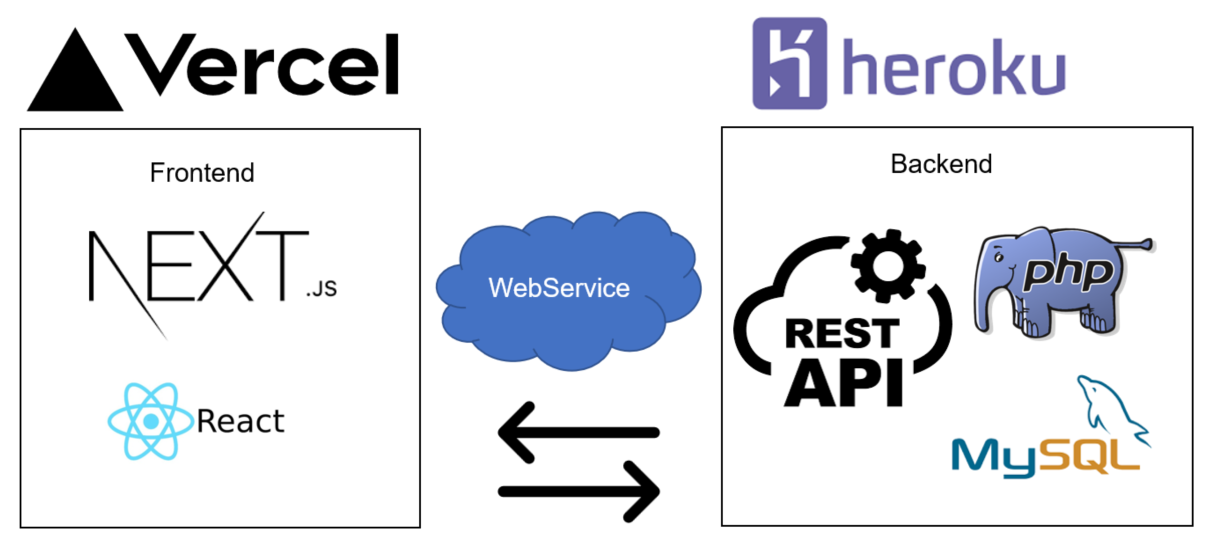
\includegraphics[scale=.33]{infografico.png}
    \vspace{5pt}
    \legend{Fonte: Próprio autor}
\end{figure}


\section{Métodos} \label{metodos}
Para este projeto, o desenvolvimento foi baseado no processo unificado, que as etapas são incrementais e interativas, mesmo sendo definido por etapas \cite{SOMMERVILE}. As etapas são definidas por: concepção, elaboração, construção e transição.

% A primeira etapa é dada pela concepção, a qual irá levantar o escopo do projeto de forma mais genérica, sendo o caso de uso, que será incrementado a cada nova funcionalidade. Este por sua vez, irá demonstrar como será a interação dos usuários, chamados de atores, com o sistema e suas funcionalidades, que são os casos de uso para cada um. Sendo assim, os atores identificados inicialmente são: supervisor, associado, usuário, visitante e o apresentador, podendo serem vistos no caso de uso representado pela figura \ref{fig_caso_uso}.

% \begin{figure}[H]
    % \caption{\label{fig_caso_uso}Caso de uso}
    % \vspace{5pt}
    % \centering
    % 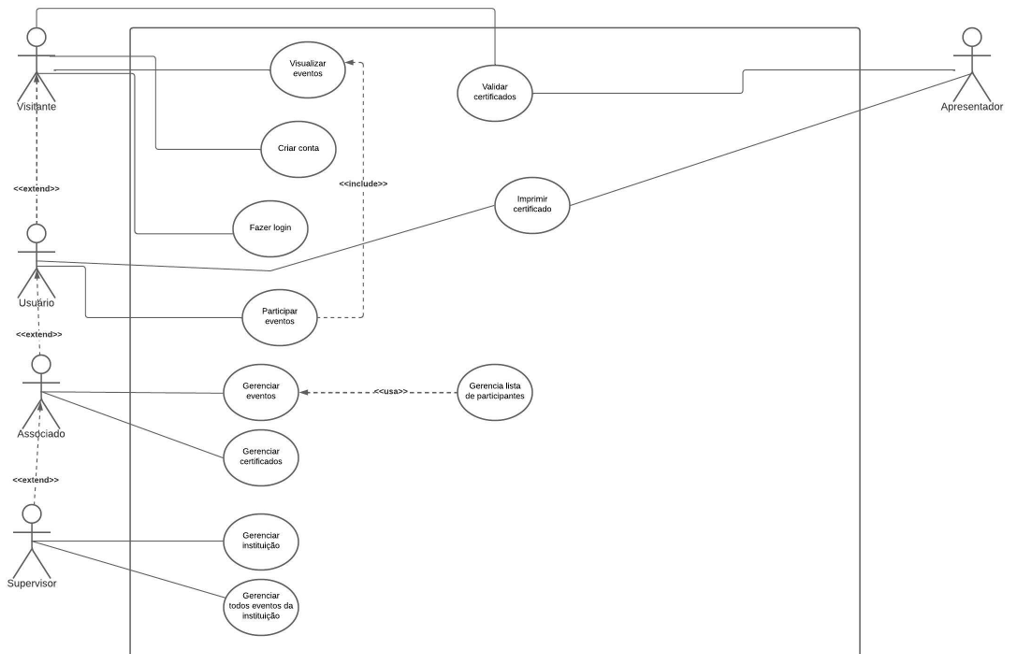
\includegraphics[scale=.4]{caso de uso.png}
    % \vspace{5pt}
    % \legend{Fonte: Próprio autor}
% \end{figure}

Há cinco níveis de acesso ao sistema, sendo estes:
\begin{itemize}
    \item \textbf{Visitante: } não possui cadastro no sistema ou não entrou em sua conta ainda, portanto seu processo estará pré-definido de forma que possa visualizar os eventos, mas não poderá participar destes. Além disso, poderá criar conta e fazer login, no que se diz a respeito do seu cadastro e por fim poderá validar os certificados de terceiros, caso tenha a chave necessária.
    \item \textbf{Usuário: }interage com o sistema de modo que poderá gerenciar seu perfil, fazendo alterações em áreas determinadas de seu cadastro. Além disso, poderá participar de eventos, os quais irão gerar certificados que poderão ser convertidos para arquivos e salvos no computador, além de serem enviados por email caso tenham participado do evento. Vale ressaltar que estas ações só poderão ser feitas após a realização do login. E para que seja feito isto, é necessário que seja feito um cadastro na aplicação utilizando-se de dados pessoais tais como: nome completo, email, CPF e telefone para que sejam gerados os certificados de forma correta. 
    \item \textbf{Apresentador: }tem como principal função, podendo ou não ter um cadastro na aplicação, ser vinculado a um evento o qual irá apresentar. Ou seja, supondo que seja uma palestra, este será o palestrante e terá acesso ao seu certificado por meio do email cadastrado no evento. Caso já tenha um cadastro, este será vinculado diretamente a conta e poderá ser impresso (sem a necessidade de consulta ao email) diretamente da aplicação.
    \item \textbf{Associado: }tem acesso a tudo que um usuário faz, mas poderá gerir até certo nível a instituição, fazendo a criação de eventos acadêmicos. Para que alguém se torne associado, é necessário que o supervisor o vincule a uma instituição. Sua principal função é gerir os eventos criados pelo próprio autor, de forma que serão vinculados a este por meio da instituição.
    \item \textbf{Supervisor: }tem a função de criar e gerir a instituição, além de gerir todos os eventos pertencentes a esta.
\end{itemize}


\subsection{API}
A API para a aplicação será feita em Laravel com utilização do SGBD MySQL por meio de uma autenticação segura. As consultas e requisições ao banco de dados serão feitas nesta camada. E seu retorno dos dados requisitados serão transmitidos ao módulo de visão via JSON.

Além disso, a autenticação da aplicação será validada por meio do JWT\footnote{JSON Web Token (JWT) é um padrão aberto (RFC 7519) que define uma maneira compacta e independente para transmitir informações com segurança entre as partes como um objeto JSON. Essas informações podem ser verificadas e confiáveis porque estão assinadas digitalmente.} a autenticidade do usuário, ou seja, para cada requisição que exija segurança, como por exemplo a criação de um evento ou alterações na conta do usuário, que dizendo de forma geral, qualquer alteração solicitada ao SGBD. Isto garantirá que o usuário está devidamente conectado, assim como que sua autenticidade.

\subsection{Frontend}
O frontend será feito em Next.js, na qual irá receber os dados referentes a API e convertê-los para uma interface ao usuário. Esta interface será um site no qual, usuário poderá interagir e fazer todas as ações permitidas. Além disso, este módulo feita de forma que seja simples, fácil empregando conceitos de usabilidade para uma melhor experiência.

Para evitar fraudes com bots, será necessário utilizar um sistema que verifique isto, principalmente na criação de usuários, assim como no login destes que é onde vem a ideia do CAPTCHA\footnote{O CAPTCHA (Teste de Turing público completamente automatizado para distinguir entre computadores e pessoas) é um tipo de medida de segurança conhecido como autenticação por desafio e resposta. O CAPTCHA protege contra spam e descriptografia de senhas com um teste simples que prova que você é um ser humano, não um computador tentando invadir uma conta protegida por senha.}. A implementação utilizada foi o hCaptcha\footnote{O hCAPTCHA é um serviço de CAPTCHA gratuito e independente que fornece desafios fáceis para humanos, entretanto são complexos para uma máquina, tais como classificação de um objeto dada as imagens.}, o qual irá proteger o sistema de login da aplicação, dificultando o acesso para máquinas automatizadas.

\subsection{Versionamento}
O versionamento foi feito utilizando o Git, por meio de um repositório no Github. Cada versão foi feita com base nos critérios do GitFlow, seguindo a lógica descrita de master e develop, sendo a primeira a versão de produção e a outra sendo a versão com as novas funcionalidades e para testes. Cada parte da aplicação terá seu versionamento de acordo com sua funcionabilidade, ou seja, a API terá seu versionamento separado do frontend.